\section{Related work}
In this section we will cover Cassandra and HBase. Two other distributed systems that are used 

\subsection{Cassandra}
Cassandra scalable NoSQL database now available as open source through the Apache foundation. It was built from scratch with goal of being a massively scalable NoSQL database. In a cluster running Cassandra there is no sense of a master node, and all communication between nodes use peer to peer and the gossip protocol. As an administrator it is easy to scale Cassandra to meet both current and future system requirements. 

\subsubsection{Reads and writes}
In Cassandra all participating nodes can be accessed for writes and reads. To ensure durability all writes are preceded by a write to a commit log. If a node has crashed, a node holding a replica will service reads and writes according to the hinted handoff strategy. As with Voldemort, Cassandra also features tunable consistency. 

\subsubsection{Data model}
The Cassandra data model is based on a key:value model, however Cassandra extends this model with up to two levels of nesting. This forms a map structure called columns where the outer row key acts as a primary key and the inner sorted map holds all information: \texttt{Map<RowKey, SortedMap<ColumnKey, ColumnValue>>}. By using maps we achieve easy lookups and range scans. By using one more level of nesting we can group columns. These are called super columns. In Cassandra de-normalization is used to be able to efficiently perform queries that accesses information stored in separate columns. To allow this composite columns can be created to match the need of one or more specific queries. These composite columns simply gather information already stored in various columns for easier access. 

\begin{figure}[h]
    \centering
    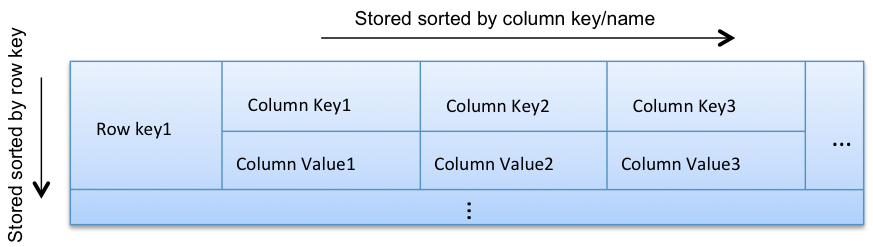
\includegraphics[width=0.5\textwidth]{resources/cas_col.png}
    \caption{A sample column. The row key acts as a primary key and each key:value pair would hold one field in a table. Images borrowed from www.ebaytechblog.com}
    \label{fig:sample_col}
\end{figure}

\begin{figure}[h]
    \centering
    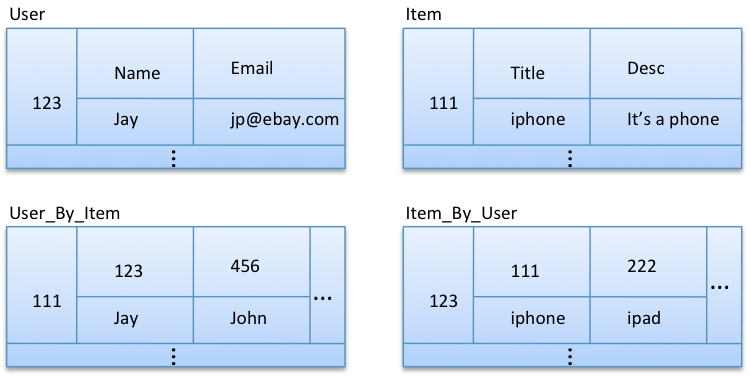
\includegraphics[width=0.6\textwidth]{resources/cas_comp_col.png}
    \caption{A sample composite columns. Here we have separate composite column to efficiently be able to serve queries on users by item and item by users.}
    \label{fig:sample_comp_col}
\end{figure}

\begin{figure}[ht]
	\centering
	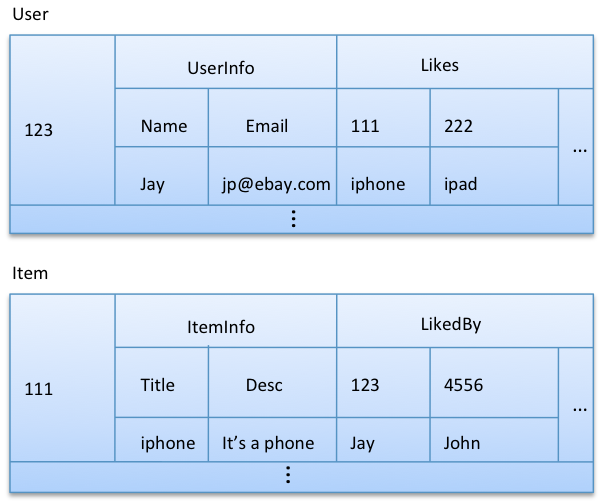
\includegraphics[width=0.4\textwidth]{resources/cas_super_col.png}
	\caption{A sample super column. Here we can see an outer map containing a person and the inner maps consisting of various composite columns}
	\label{fig:sample_super_col}
\end{figure}

Cassandra is used by several well known companies. Netflix uses Cassandra for several applications, including its subscriber system and viewer history service. Facebook used Cassandra to power their inbox search, however this was abandoned in late 2010 in favor of HBase. Spotify also migrated to Cassandra after migrating away from postgreSQL because of scaling issues. They use Cassandra to store playlists, radio stations and notification notifications.

\subsection{HBase}
HBase is based on Googles paper on BigTable.
It is a sparse, distributed, persistent multi-dimensional sorted map.

With regards to the CAP-theorem (Consistency, Availability, Partitioning), HBase provides consistency and tolerance to partitioning, making HBase fault tolerant and easy to reason with in practice.

Important to note is that HBase provides a sparse multi-dimensional \emph{sorted} map.
Keys in the table are sorted, such that similar items are close to another when scanning a table.

E.g. when storing data about urls, the keys are written in reverse: \texttt{com.google.www/users}. This scheme keeps urls from the same domain and subdomain close to each other in the sorted map.

The \emph{rows} or \emph{entries} are typically sparse, meaning that most of the columns, in the table are empty.

To visualize a HBase record, it can help to think of a map of maps:

\begin{lstlisting}
{
	"com.google.www/account": {
		"family": {
			"special": "value"
		},
		"anchor": {
			"com.cnn.www": "value"
		}
	}
	"com.google.www/users": {
		"family": {
			"": "value"
		},
		"anchor": {
			"no.nrk.www": "value"
		}
	}
}
\end{lstlisting}

The families for a record is static for the table at creation, but every family can hold any number of columns within, even many or none.
This is where the sparse property comes from, as most entries will not have a value for the set of all sub-families in the table, leaving most column values empty.

Every \emph{row} or \emph{entry} also has an associated timestamp, used for versioning. This is typically a monotonically increasing number, such as seconds since \emph{epoch}. HBase stores a given number of versions of an entry, and can be queried for these. 
These different versions are stored in descending order, such that the highest number entry, i.e. the newest, is the first entry.

This gives a possible query structure as such \texttt{<key, family:column, timestamp>}. Timestamp is optional. If no timestamp is given, the newest entry is returned. 
If the query has a timestamp, the record with version equal to or less than the given timestamp is returned. If there is no such record, null is returned.

I.e. if we have a query \texttt{<no.nrk.www, referrals:no.nrkbeta.www, 999>}, and we have records in the database:
\begin{lstlisting}
<no.nrk.www, referrals:no.nrkbeta.www, 1001>
<no.nrk.www, referrals:no.nrkbeta.www, 777>
\end{lstlisting}
\texttt{<no.nrk.www, referrals:no.nrkbeta.www, 777>} will be returned.

\subsection{Bone dry servey that explains performance}
